\begin{enumerate}[label=\thesubsection.\arabic*,ref=\thesubsection.\theenumi]

\item Find the coordinates of the point which divides the join of $(-1,7) \text{ and } (4,-3)$ in the ratio 2:3.
	\\
		\solution
	Using section formula \eqref{eq:section_formula}, the desired point is
\begin{align}
\frac{1}{1+\frac{3}{2}}  \myvec{\myvec{
4\\
-3
}
  +
   \frac{3}{2}\myvec{
-1\\
7
}}
=\myvec{
1\\
3
}
\end{align}
See 
\figref{fig:chapters/10/7/2/1/Fig}
\begin{figure}[H]
\begin{center}
   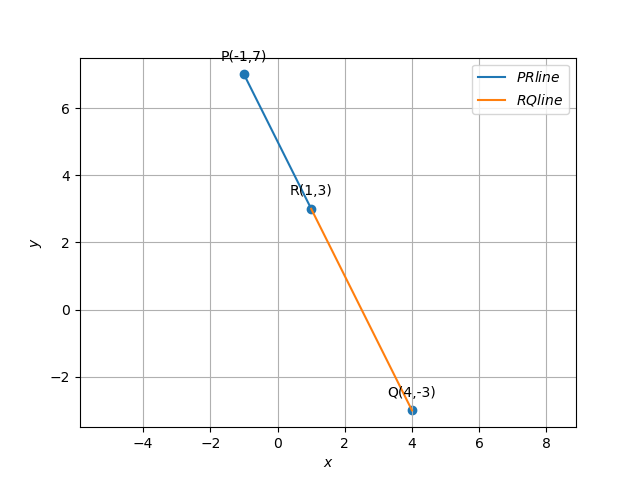
\includegraphics[width=0.75\columnwidth]{chapters/10/7/2/1/figs/linefig.png}
\end{center}
\caption{}
\label{fig:chapters/10/7/2/1/Fig}
\end{figure}


\item Find the coordinates of the points of trisection of the line segment joining $(4,-1)$  and  $(-2,3)$.
	\\
		\solution
	Using section formula,
\begin{align}
\vec{R}=\frac{1}{1+\frac{1}{2}}\brak{\myvec{4\\-1}+\frac{1}{2}\myvec{-2\\-3}}
=\myvec{2\\ \frac{-5}{3}}\\
\vec{S}=\frac{1}{1+\frac{2}{1}}\brak{\myvec{4\\-1}+\frac{2}{1}\myvec{-2\\-3}}
=\myvec{0\\ \frac{-7}{3}}
\end{align}
which are the desired points of trisection.
\iffalse
See
		\figref{fig:chapters/10/7/2/2/Figure}
\begin{figure}[H]
\centering
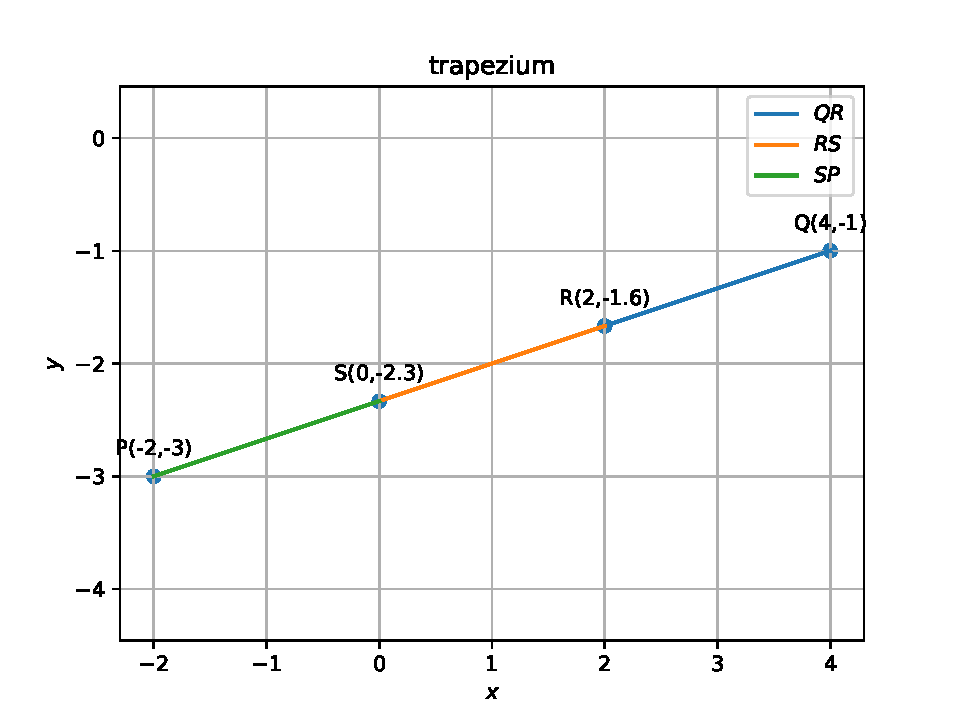
\includegraphics[width=0.75\columnwidth]{chapters/10/7/2/2/figs/dj.pdf}
\caption{}
		\label{fig:chapters/10/7/2/2/Figure}
\end{figure}
\fi

\item Find the ratio in which the line segment joining the points $(-3,10) \text{ and } (6,-8)$ $\text{ is divided by } (-1,6)$.
	\\
		\solution
	\iffalse
\documentclass[12pt]{article}
\usepackage{graphicx}
%\documentclass[journal,12pt,twocolumn]{IEEEtran}
\usepackage[none]{hyphenat}
\usepackage{graphicx}
\usepackage{listings}
\usepackage[english]{babel}
\usepackage{graphicx}
\usepackage{caption} 
\usepackage{hyperref}
\usepackage{booktabs}
\def\inputGnumericTable{}
\usepackage{color}                                            %%
    \usepackage{array}                                            %%
    \usepackage{longtable}                                        %%
    \usepackage{calc}                                             %%
    \usepackage{multirow}                                         %%
    \usepackage{hhline}                                           %%
    \usepackage{ifthen}
\usepackage{array}
\usepackage{amsmath}   % for having text in math mode
\usepackage{listings}
\lstset{
language=tex,
frame=single, 
breaklines=true
}
  
%Following 2 lines were added to remove the blank page at the beginning
\usepackage{atbegshi}% http://ctan.org/pkg/atbegshi
\AtBeginDocument{\AtBeginShipoutNext{\AtBeginShipoutDiscard}}
%
%New macro definitions
\newcommand{\mydet}[1]{\ensuremath{\begin{vmatrix}#1\end{vmatrix}}}
\providecommand{\brak}[1]{\ensuremath{\left(#1\right)}}
\providecommand{\norm}[1]{\left\lVert#1\right\rVert}
\newcommand{\solution}{\noindent \textbf{Solution: }}
\newcommand{\myvec}[1]{\ensuremath{\begin{pmatrix}#1\end{pmatrix}}}
\let\vec\mathbf
\begin{document}
\begin{center}
\title{\textbf{Coordinate Geometry}}
\date{\vspace{-5ex}} %Not to print date automatically
\maketitle
\end{center}
\setcounter{page}{1}
\section*{10$^{th}$ Maths - Chapter 7}
This is Problem-4 from Exercise 7.2
\begin{enumerate}
\item Find the ratio in which the line segement joining the points $\myvec{-3 \\ 10}$ and $\myvec{6\\-8}$ is divided by $\myvec{-1\\6}$.\\
\solution \\
\fi
		The input parameters for this problem are available in Table \eqref{tab:10/7/2/4-1}.
\begin{table}[ht!]
%%%%%%%%%%%%%%%%%%%%%%%%%%%%%%%%%%%%%%%%%%%%%%%%%%%%%%%%%%%%%%%%%%%%%%
%%                                                                  %%
%%  This is the header of a LaTeX2e file exported from Gnumeric.    %%
%%                                                                  %%
%%  This file can be compiled as it stands or included in another   %%
%%  LaTeX document. The table is based on the longtable package so  %%
%%  the longtable options (headers, footers...) can be set in the   %%
%%  preamble section below (see PRAMBLE).                           %%
%%                                                                  %%
%%  To include the file in another, the following two lines must be %%
%%  in the including file:                                          %%
%%        \def\inputGnumericTable{}                                 %%
%%  at the beginning of the file and:                               %%
%%        \input{name-of-this-file.tex}                             %%
%%  where the table is to be placed. Note also that the including   %%
%%  file must use the following packages for the table to be        %%
%%  rendered correctly:                                             %%
%%    \usepackage[latin1]{inputenc}                                 %%
%%    \usepackage{color}                                            %%
%%    \usepackage{array}                                            %%
%%    \usepackage{longtable}                                        %%
%%    \usepackage{calc}                                             %%
%%    \usepackage{multirow}                                         %%
%%    \usepackage{hhline}                                           %%
%%    \usepackage{ifthen}                                           %%
%%  optionally (for landscape tables embedded in another document): %%
%%    \usepackage{lscape}                                           %%
%%                                                                  %%
%%%%%%%%%%%%%%%%%%%%%%%%%%%%%%%%%%%%%%%%%%%%%%%%%%%%%%%%%%%%%%%%%%%%%%



%%  This section checks if we are begin input into another file or  %%
%%  the file will be compiled alone. First use a macro taken from   %%
%%  the TeXbook ex 7.7 (suggestion of Han-Wen Nienhuys).            %%
\def\ifundefined#1{\expandafter\ifx\csname#1\endcsname\relax}


%%  Check for the \def token for inputed files. If it is not        %%
%%  defined, the file will be processed as a standalone and the     %%
%%  preamble will be used.                                          %%
\ifundefined{inputGnumericTable}

%%  We must be able to close or not the document at the end.        %%
 \def\gnumericTableEnd{\end{document}}


%%%%%%%%%%%%%%%%%%%%%%%%%%%%%%%%%%%%%%%%%%%%%%%%%%%%%%%%%%%%%%%%%%%%%%
%%                                                                  %%
%%  This is the PREAMBLE. Change these values to get the right      %%
%%  paper size and other niceties.                                  %%
%%                                                                  %%
%%%%%%%%%%%%%%%%%%%%%%%%%%%%%%%%%%%%%%%%%%%%%%%%%%%%%%%%%%%%%%%%%%%%%%

 \documentclass[12pt%
     %,landscape%
                    ]{report}
       \usepackage[latin1]{inputenc}
       \usepackage{fullpage}
       \usepackage{color}
       \usepackage{array}
       \usepackage{longtable}
       \usepackage{calc}
       \usepackage{multirow}
       \usepackage{hhline}
       \usepackage{ifthen}

 \begin{document}


%%  End of the preamble for the standalone. The next section is for %%
%%  documents which are included into other LaTeX2e files.          %%
\else

%%  We are not a stand alone document. For a regular table, we will %%
%%  have no preamble and only define the closing to mean nothing.   %%
    \def\gnumericTableEnd{}

%%  If we want landscape mode in an embedded document, comment out  %%
%%  the line above and uncomment the two below. The table will      %%
%%  begin on a new page and run in landscape mode.                  %%
%       \def\gnumericTableEnd{\end{landscape}}
%       \begin{landscape}


%%  End f theoelse clause for this file being \input.              %%
\fi

%%%%%%%%%%%%%%%%%%%%%%%%%%%%%%%%%%%%%%%%%%%%%%%%%%%%%%%%%%%%%%%%%%%%%%
%%                                                                  %%
%%  The rest is the gnumeric table, except for the closing          %%
%%  statement. Changes below will alter the table's appearance.     %%
%%                                                                  %%
%%%%%%%%%%%%%%%%%%%%%%%%%%%%%%%%%%%%%%%%%%%%%%%%%%%%%%%%%%%%%%%%%%%%%%

\providecommand{\gnumericmathit}[1]{#1} 
%%  Uncomment the next line if you would like your numbers to be in %%
%%  italics if they are italizised in the gnumeric table.           %%
%\renewcommand{\gnumericmathit}[1]{\mathit{#1}}
\providecommand{\gnumericPB}[1]%
{\let\gnumericTemp=\\#1\let\\=\gnumericTemp\hspace{0pt}}
 \ifundefined{gnumericTableWidthDefined}
        \newlength{\gnumericTableWidth}
        \newlength{\gnumericTableWidthComplete}
        \newlength{\gnumericMultiRowLength}
        \global\def\gnumericTableWidthDefined{}
 \fi
%% The following setting protects this code from babel shorthands.  %%
 \ifthenelse{\isundefined{\languageshorthands}}{}{\languageshorthands{english}}
%%  The default table format retains the relative column widths of  %%
%%  gnumeric. They can easily be changed to c, r or l. In that case %%
%%  you may want to comment out the next line and uncomment the one %%
%%  thereafter                                                      %%
\providecommand\gnumbox{\makebox[0pt]}
%%\providecommand\gnumbox[1][]{\makebox}

%% to adjust positions in multirow situations                       %%
\setlength{\bigstrutjot}{\jot}
\setlength{\extrarowheight}{\doublerulesep}

%%  The \setlongtables command keeps column widths the same across  %%
%%  pages. Simply comment out next line for varying column widths.  %%
\setlongtables

\setlength\gnumericTableWidth{%
 53pt+%
 53pt+%
 82pt+%
 53pt+%
0pt}
\def\gumericNumCols{4}
\setlength\gnumericTableWidthComplete{\gnumericTableWidth+%
         \tabcolsep*\gumericNumCols*2+\arrayrulewidth*\gumericNumCols}
\ifthenelse{\lengthtest{\gnumericTableWidthComplete > \linewidth}}%
         {\def\gnumericScale{1*\ratio{\linewidth-%
                        \tabcolsep*\gumericNumCols*2-%
                        \arrayrulewidth*\gumericNumCols}%
{\gnumericTableWidth}}}%
{\def\gnumericScale{1}}

%%%%%%%%%%%%%%%%%%%%%%%%%%%%%%%%%%%%%%%%%%%%%%%%%%%%%%%%%%%%%%%%%%%%%%
%%                                                                  %%
%% The following are the widths of the various columns. We are      %%
%% defining them here because then they are easier to change.       %%
%% Depending on the cell formats we may use them more than once.    %%
%%                                                                  %%
%%%%%%%%%%%%%%%%%%%%%%%%%%%%%%%%%%%%%%%%%%%%%%%%%%%%%%%%%%%%%%%%%%%%%%

\ifthenelse{\isundefined{\gnumericColA}}{\newlength{\gnumericColA}}{}\settowidth{\gnumericColA}{\begin{tabular}{@{}p{53pt*\gnumericScale}@{}}x\end{tabular}}
\ifthenelse{\isundefined{\gnumericColB}}{\newlength{\gnumericColB}}{}\settowidth{\gnumericColB}{\begin{tabular}{@{}p{53pt*\gnumericScale}@{}}x\end{tabular}}
\ifthenelse{\isundefined{\gnumericColC}}{\newlength{\gnumericColC}}{}\settowidth{\gnumericColC}{\begin{tabular}{@{}p{82pt*\gnumericScale}@{}}x\end{tabular}}
\ifthenelse{\isundefined{\gnumericColD}}{\newlength{\gnumericColD}}{}\settowidth{\gnumericColD}{\begin{tabular}{@{}p{53pt*\gnumericScale}@{}}x\end{tabular}}

\begin{center}
\begin{tabular}[c]{%
 b{\gnumericColA}%
 b{\gnumericColB}%
 b{\gnumericColC}%
 b{\gnumericColD}%
 }

%%%%%%%%%%%%%%%%%%%%%%%%%%%%%%%%%%%%%%%%%%%%%%%%%%%%%%%%%%%%%%%%%%%%%%
%%  The longtable options. (Caption, headers... see Goosens, p.124) %%
% \caption{The Table Caption.}             \\ %
% \hline % Across the top of the table.
%%  The rest of these options are table rows which are placed on    %%
%%  the first, last or every page. Use \multicolumn if you want.    %%

%%  Header for the first page.                                      %%
% \multicolumn{4}{c}{The First Header} \\ \hline 
% \multicolumn{1}{c}{colTag} %Column 1
% &\multicolumn{1}{c}{colTag} %Column 2
% &\multicolumn{1}{c}{colTag} %Column 3
% &\multicolumn{1}{c}{colTag} \\ \hline %Last column
% \endfirsthead

%%  The running header definition.                                  %%
% \hline
% \multicolumn{4}{l}{\ldots\small\slshape continued} \\ \hline
% \multicolumn{1}{c}{colTag} %Column 1
% &\multicolumn{1}{c}{colTag} %Column 2
% &\multicolumn{1}{c}{colTag} %Column 3
% &\multicolumn{1}{c}{colTag} \\ \hline %Last column
% \endhead

%%  The running footer definition.                                  %%
% \hline
% \multicolumn{4}{r}{\small\slshape continued\ldots} \\
% \endfoot

%%  The ending footer definition.                                   %%
% \multicolumn{4}{c}{That's all folks} \\ \hline 
% \endlastfoot
%%%%%%%%%%%%%%%%%%%%%%%%%%%%%%%%%%%%%%%%%%%%%%%%%%%%%%%%%%%%%%%%%%%%%%

\hhline{|-|-|-~}
  \multicolumn{1}{|p{\gnumericColA}|}%
 {\gnumericPB{\centering}\gnumbox{\textbf{Symbol}}}
 &\multicolumn{1}{p{\gnumericColB}|}%
 {\gnumericPB{\centering}\gnumbox{\textbf{Value}}}
 &\multicolumn{1}{p{\gnumericColC}|}%
 {\gnumericPB{\centering}\gnumbox{\textbf{Description}}}
 &
\\
\hhline{|---|~}
  \multicolumn{1}{|p{\gnumericColA}|}%
 {\gnumericPB{\centering}\gnumbox{$\vec{P}$}}
 &\multicolumn{1}{p{\gnumericColB}|}%
 {\gnumericPB{\centering}\gnumbox{$\myvec{-3\\10}$}}
 &\multicolumn{1}{p{\gnumericColC}|}%
 {\gnumericPB{\centering}\gnumbox{First point}}
 &
\\
\hhline{|---|~}
  \multicolumn{1}{|p{\gnumericColA}|}%
 {\gnumericPB{\centering}\gnumbox{$\vec{Q}$}}
 &\multicolumn{1}{p{\gnumericColB}|}%
 {\gnumericPB{\centering}\gnumbox{$\myvec{6\\-8}$}}
 &\multicolumn{1}{p{\gnumericColC}|}%
 {\gnumericPB{\centering}\gnumbox{Second point}}
 &
\\
\hhline{|---|~}
  \multicolumn{1}{|p{\gnumericColA}|}%
 {\gnumericPB{\centering}\gnumbox{$\vec{R}$}}
 &\multicolumn{1}{p{\gnumericColB}|}%
 {\gnumericPB{\centering}\gnumbox{$\myvec{-1\\6}$}}
 &\multicolumn{1}{p{\gnumericColC}|}%
 {\gnumericPB{\centering}\gnumbox{Desired point}}
 &
\\
\hhline{|-|-|-|~}
\end{tabular}
 \end{center}

\ifthenelse{\isundefined{\languageshorthands}}{}{\languageshorthands{\languagename}}
\gnumericTableEnd

\caption{}
\label{tab:10/7/2/4-1} 
\end{table}
Using section formula,
\begin{align}
         \vec{R} &=\frac{\vec{Q}+n\vec{P}}{1+n}\label{eq:chapters/10/7/2/4/1}
\end{align}
Substituting the values of $\vec{P},\vec{Q}$ and $\vec{R}$ in \eqref{eq:chapters/10/7/2/4/1}
\begin{align}
         \myvec{-1\\6} &=\frac{{\myvec{-3\\10}+n\myvec{6\\-8}}}{1+n}\\
 &=\frac{1}{1+n}\brak{{\myvec{-3\\10}+n\myvec{6\\-8}}} \\
 &=\frac{1}{1+n}\myvec{-3+6n\\10-8n} \label{eq:chapters/10/7/2/4/4}
\end{align}
Simplifying \eqref{eq:chapters/10/7/2/4/4} yeilds,
\begin{align}
          -1 &=\frac{-3+6n}{1+n}\\
\implies          n &=\frac{2}{7}
\end{align}
Also,
\begin{align}
          6 &=\frac{10-8n}{1+n}\\
    \implies      n &=\frac{2}{7}
\end{align}
Hence the desired ratio is $\dfrac{2}{7}$.  
\begin{figure}[!h]
 \begin{center}
  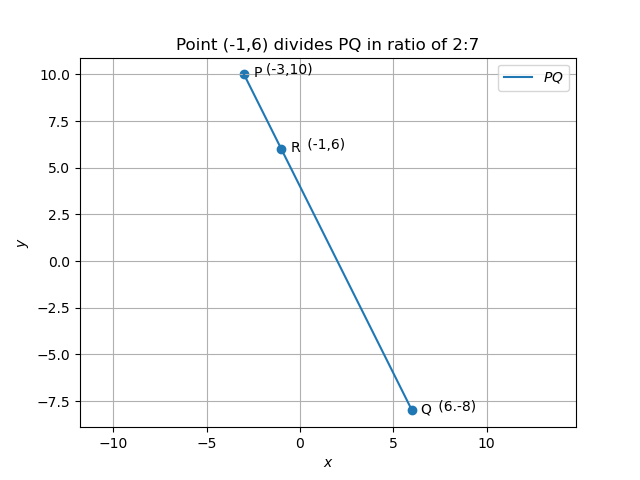
\includegraphics[width=\columnwidth]{chapters/10/7/2/4/figs/fig.png}
 \end{center}
\caption{}
\label{fig:10/7/2/4Fig1}
\end{figure}

\item Find the coordinates of a point $A$, where $AB$ is the diameter of a circle whose centre is $ C(2,-3)$  and  $B$ is $(1,4)$.
	\\
		\solution
		\begin{align}
	\vec{C} = \frac{\vec{A+B}}{2} 
	\implies 	\vec{A} = 2\vec{C}-\vec{B} 
	 = \myvec{3\\-10\\}	
	\end{align}       
	The radius is then obtained as
\begin{align}
	\norm{\vec{B}-\vec{C}} = 5\sqrt{2}
\end{align}
	See 
\figref{fig:chapters/10/7/2/7Fig}.
\begin{figure}[H]
\begin{center}	
	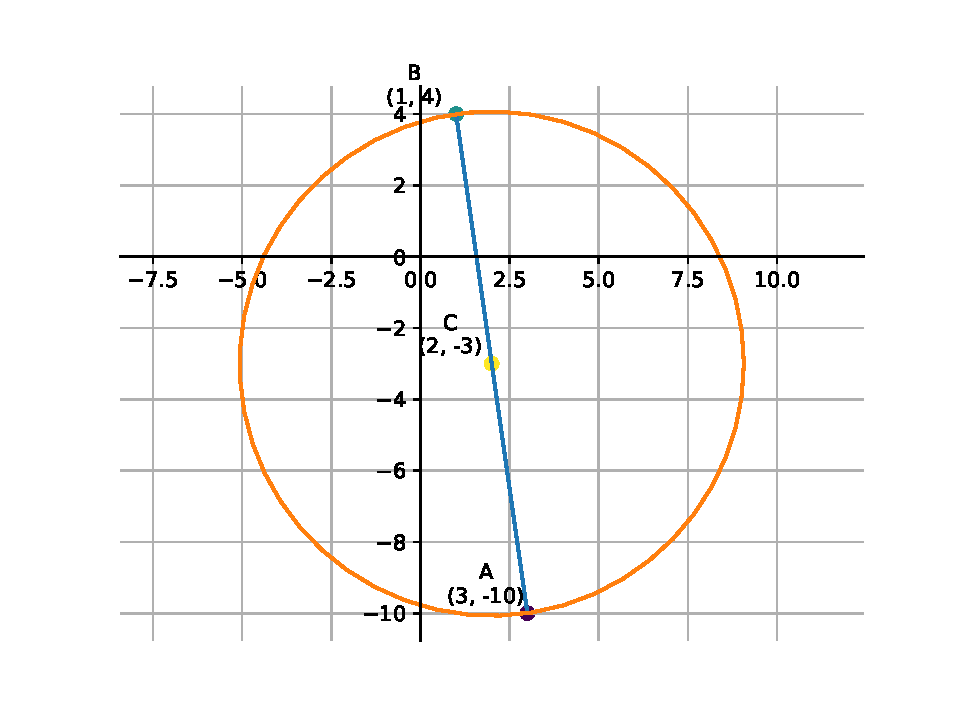
\includegraphics[width=0.75\columnwidth]{chapters/10/7/2/7/figs/fig.pdf}
\end{center}
\caption{}
\label{fig:chapters/10/7/2/7Fig}
\end{figure}
	

\item If $A$ and  $B$ are $(-2,-2)$ and  $(2,-4)$, respectively, find the coordinates of $P$ such that $AP= \frac {3}{7}AB$  and $ P$ lies on the line segment $AB$.
	\\
		\solution
	Using section formula, 
\begin{align}
\vec{P}&=\frac{1}{1+\frac{3}{4}}\brak{\myvec{-2\\-2}+\frac{3}{4}\myvec{2\\-4}}
=\myvec{\frac{-2}{7}\\[1pt] \frac{-20}{7}}
\end{align}
\iffalse
See 
   \figref{fig:chapters/10/7/2/8/vec.png}.
\begin{figure}
   \centering 
 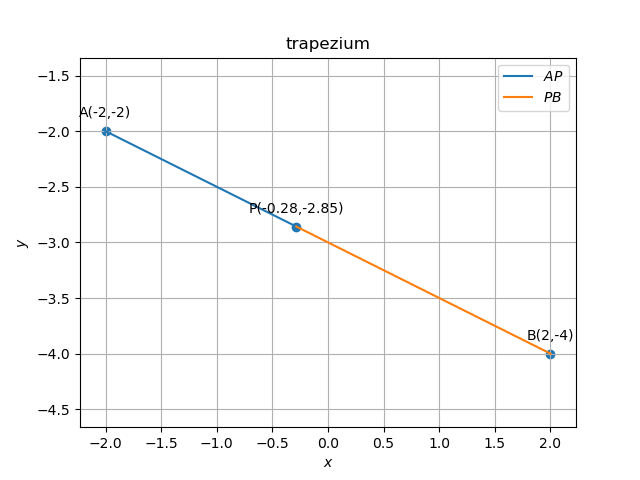
\includegraphics[width=0.75\columnwidth]{chapters/10/7/2/8/figs/vec.png}
   \caption{}
   \label{fig:chapters/10/7/2/8/vec.png}
   \end{figure}
   \fi

\item Find the coordinates of the points which divide the line segment joining $A(-2,2)$  and  $B(2,8)$ into four equal parts.
	\\
		\solution
	Using section formula,
\begin{align}
	\vec{R}_k=\frac{\vec{B}+k\vec{A}}{1+k}, k = \frac{i}{n-i}, 0 < i < n
\end{align}
for $n = 4$.
See 
\figref{fig:chapters/10/7/2/9/Fig}.
\begin{figure}[H]
\begin{center}
   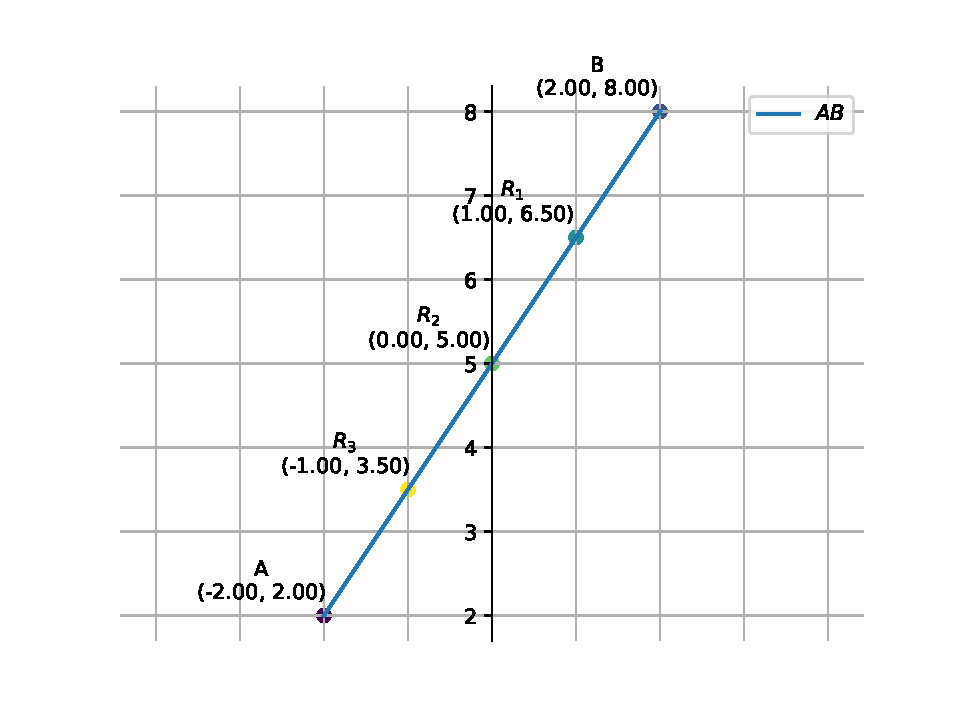
\includegraphics[width=0.75\columnwidth]{chapters/10/7/2/9/figs/fig.pdf}
\end{center}
\caption{}
\label{fig:chapters/10/7/2/9/Fig}
\end{figure}


\item Find the position vector of a point $\vec{R}$ which divides the line joining two points $\vec{P}$
and $\vec{Q}$ whose position vectors are $\hat{i}+2\hat{j}-\hat{k}$ and $-\hat{i}+\hat{j}+\hat{k}$ respectively, in the
ratio 2 : 1
\begin{enumerate}
    \item  internally
    \item  externally
\end{enumerate}
\solution
		\iffalse
\documentclass[journal,12pt,twocolumn]{IEEEtran}
%
\usepackage{setspace}
\usepackage{gensymb}
%\doublespacing
\singlespacing

%\usepackage{graphicx}
%\usepackage{amssymb}
%\usepackage{relsize}
\usepackage[cmex10]{amsmath}
%\usepackage{amsthm}
%\interdisplaylinepenalty=2500
%\savesymbol{iint}
%\usepackage{txfonts}
%\restoresymbol{TXF}{iint}
%\usepackage{wasysym}
\usepackage{amsthm}
%\usepackage{iithtlc}
\usepackage{mathrsfs}
\usepackage{txfonts}
\usepackage{stfloats}
\usepackage{bm}
\usepackage{cite}
\usepackage{cases}
\usepackage{subfig}
%\usepackage{xtab}
\usepackage{longtable}
\usepackage{multirow}
%\usepackage{algorithm}
%\usepackage{algpseudocode}
\usepackage{enumitem}
\usepackage{mathtools}
\usepackage{steinmetz}
\usepackage{tikz}
\usepackage{circuitikz}
\usepackage{verbatim}
\usepackage{tfrupee}
\usepackage[breaklinks=true]{hyperref}
%\usepackage{stmaryrd}
\usepackage{tkz-euclide} % loads  TikZ and tkz-base
%\usetkzobj{all}
\usetikzlibrary{calc,math}
\usepackage{listings}
    \usepackage{color}                                            %%
    \usepackage{array}                                            %%
    \usepackage{longtable}                                        %%
    \usepackage{calc}                                             %%
    \usepackage{multirow}                                         %%
    \usepackage{hhline}                                           %%
    \usepackage{ifthen}                                           %%
  %optionally (for landscape tables embedded in another document): %%
    \usepackage{lscape}     
\usepackage{multicol}
\usepackage{chngcntr}
%\usepackage{enumerate}
\usepackage{graphicx}

%\usepackage{wasysym}
%\newcounter{MYtempeqncnt}
\DeclareMathOperator*{\Res}{Res}
%\renewcommand{\baselinestretch}{2}
\renewcommand\thesection{\arabic{section}}
\renewcommand\thesubsection{\thesection.\arabic{subsection}}
\renewcommand\thesubsubsection{\thesubsection.\arabic{subsubsection}}

\renewcommand\thesectiondis{\arabic{section}}
\renewcommand\thesubsectiondis{\thesectiondis.\arabic{subsection}}
\renewcommand\thesubsubsectiondis{\thesubsectiondis.\arabic{subsubsection}}

% correct bad hyphenation here
\hyphenation{op-tical net-works semi-conduc-tor}
\def\inputGnumericTable{}                                 %%

\lstset{
%language=C,
frame=single, 
breaklines=true,
columns=fullflexible
}
%\lstset{
%language=tex,
%frame=single, 
%breaklines=true
%}

\begin{document}
%


\newtheorem{theorem}{Theorem}[section]
\newtheorem{problem}{Problem}
\newtheorem{proposition}{Proposition}[section]
\newtheorem{lemma}{Lemma}[section]
\newtheorem{corollary}[theorem]{Corollary}
\newtheorem{example}{Example}[section]
\newtheorem{definition}[problem]{Definition}
%\newtheorem{thm}{Theorem}[section] 
%\newtheorem{defn}[thm]{Definition}
%\newtheorem{algorithm}{Algorithm}[section]
%\newtheorem{cor}{Corollary}
\newcommand{\BEQA}{\begin{eqnarray}}
\newcommand{\EEQA}{\end{eqnarray}}
\newcommand{\define}{\stackrel{\triangle}{=}}

\bibliographystyle{IEEEtran}
%\bibliographystyle{ieeetr}


\providecommand{\mbf}{\mathbf}
\providecommand{\pr}[1]{\ensuremath{\Pr\left(#1\right)}}
\providecommand{\qfunc}[1]{\ensuremath{Q\left(#1\right)}}
\providecommand{\sbrak}[1]{\ensuremath{{}\left[#1\right]}}
\providecommand{\lsbrak}[1]{\ensuremath{{}\left[#1\right.}}
\providecommand{\rsbrak}[1]{\ensuremath{{}\left.#1\right]}}
\providecommand{\brak}[1]{\ensuremath{\left(#1\right)}}
\providecommand{\lbrak}[1]{\ensuremath{\left(#1\right.}}
\providecommand{\rbrak}[1]{\ensuremath{\left.#1\right)}}
\providecommand{\cbrak}[1]{\ensuremath{\left\{#1\right\}}}
\providecommand{\lcbrak}[1]{\ensuremath{\left\{#1\right.}}
\providecommand{\rcbrak}[1]{\ensuremath{\left.#1\right\}}}
\theoremstyle{remark}
\newtheorem{rem}{Remark}
\newcommand{\sgn}{\mathop{\mathrm{sgn}}}
\providecommand{\abs}[1]{\left\vert#1\right\vert}
\providecommand{\res}[1]{\Res\displaylimits_{#1}} 
\providecommand{\norm}[1]{\left\lVert#1\right\rVert}
%\providecommand{\norm}[1]{\lVert#1\rVert}
\providecommand{\mtx}[1]{\mathbf{#1}}
\providecommand{\mean}[1]{E\left[ #1 \right]}
\providecommand{\fourier}{\overset{\mathcal{F}}{ \rightleftharpoons}}
%\providecommand{\hilbert}{\overset{\mathcal{H}}{ \rightleftharpoons}}
\providecommand{\system}{\overset{\mathcal{H}}{ \longleftrightarrow}}
	%\newcommand{\solution}[2]{\textbf{Solution:}{#1}}
\newcommand{\solution}{\noindent \textbf{Solution: }}
\newcommand{\cosec}{\,\text{cosec}\,}
\providecommand{\dec}[2]{\ensuremath{\overset{#1}{\underset{#2}{\gtrless}}}}
\newcommand{\myvec}[1]{\ensuremath{\begin{pmatrix}#1\end{pmatrix}}}
\newcommand{\mydet}[1]{\ensuremath{\begin{vmatrix}#1\end{vmatrix}}}
%\numberwithin{equation}{section}
\numberwithin{equation}{subsection}
%\numberwithin{problem}{section}
%\numberwithin{definition}{section}
\makeatletter
\@addtoreset{figure}{problem}
\makeatother

\let\StandardTheFigure\thefigure
\let\vec\mathbf
%\renewcommand{\thefigure}{\theproblem.\arabic{figure}}
\renewcommand{\thefigure}{\theproblem}
%\setlist[enumerate,1]{before=\renewcommand\theequation{\theenumi.\arabic{equation}}
%\counterwithin{equation}{enumi}


%\renewcommand{\theequation}{\arabic{subsection}.\arabic{equation}}

\def\putbox#1#2#3{\makebox[0in][l]{\makebox[#1][l]{}\raisebox{\baselineskip}[0in][0in]{\raisebox{#2}[0in][0in]{#3}}}}
     \def\rightbox#1{\makebox[0in][r]{#1}}
     \def\centbox#1{\makebox[0in]{#1}}
     \def\topbox#1{\raisebox{-\baselineskip}[0in][0in]{#1}}
     \def\midbox#1{\raisebox{-0.5\baselineskip}[0in][0in]{#1}}

\vspace{3cm}

\title{EE2802: Assignment2}
\author{Nikam Pratik Balasaheb}





% make the title area
\maketitle

\newpage

%\tableofcontents

\bigskip

\renewcommand{\thefigure}{\theenumi}
\renewcommand{\thetable}{\theenumi}
%\renewcommand{\theequation}{\theenumi}

\section{Problem}
Find the position vector of a point R which divides the line joining two points P = $\myvec{1\\ 2 \\-1}$ and Q = $\myvec{ -1\\1\\1 }$ in the ratio 2:1 
\begin{enumerate}
\item internally
\item externally
\end{enumerate}

\section{Solution}

\begin{align}
\vec{P} = \myvec{ 1\\2\\-1} \\
 \vec{Q} = \myvec{ -1\\1\\1}
\end{align}

\fi

\begin{enumerate}


\item When $\vec{R}$ divides line segment joining $\vec{P}$ and $\vec{Q}$ internally,
\begin{align}
\vec{R} &= \frac{2 \vec{P} + 1 \vec{Q}}{3} \\
 &= \frac{2}{3} \vec{P} + \frac{1}{3} \vec{Q}\\
\vec{R} &= \myvec{\frac{1}{3}\\[1pt] \frac{5}{3} \\[1pt] \frac{-1}{3}}
\end{align}

\item When $\vec{R}$ divides line segment joining $\vec{P}$ and $\vec{Q}$ externally,
\begin{align}
\vec{R} &= 2 \vec{Q} - \vec{P} \\
 &= 2 \myvec{ -1\\1\\1} - \myvec{ 1\\2\\-1}\\
\vec{R} &= \myvec{ -3\\ 0 \\ 3 }
\end{align}


\end{enumerate}
See Fig. 
\ref{fig:chapters/12/10/2/15/}.
\begin{figure}[!ht]
\centering
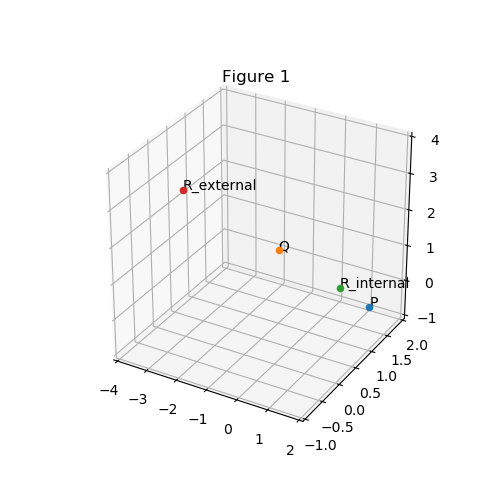
\includegraphics[width=\columnwidth]{chapters/12/10/2/15/figs/Figure_1.png}
\caption{}
\label{fig:chapters/12/10/2/15/}
\end{figure}



\item Find the position vector of the mid point of the vector joining the points $\vec{P}$(2, 3, 4)
and $\vec{Q}$(4, 1, –2).
\\
\solution
		The desired vector is
\begin{align}
\frac{1}{2}\myvec{2\\3\\4} +  \frac{1}{2}\myvec{4\\1\\-2} =\myvec{3\\2\\1} 
\end{align}




\item Determine the ratio in which the line $2x+y  - 4=0$ divides the line segment joining the points  $\vec{A}(2, - 2)$  and  $\vec{B}(3, 7)$.
\\
\solution
	\iffalse
\documentclass[journal,12pt,twocolumn]{IEEEtran}
\usepackage{graphicx}
\graphicspath{{./chapters/10/7/4/1/figs/}}{}
\usepackage{amsmath,amssymb,amsfonts,amsthm}
\newcommand{\myvec}[1]{\ensuremath{\begin{pmatrix}#1\end{pmatrix}}}
\providecommand{\norm}[1]{\lVert#1\rVert}
\usepackage{listings}
\usepackage{watermark}
\usepackage{titlesec}
\usepackage{caption}
\let\vec\mathbf
\lstset{
frame=single, 
breaklines=true,
columns=fullflexible
}
\thiswatermark{\centering \put(0,-105.0){
\includegraphics[scale=0.15]{/sdcard/IITH/vector/vectpr-4/chapters/10/7/4/1/figs/logo.png}} }
\title{\mytitle}
\title{
Assignment - Vector-4
}
\author{Surajit Sarkar}
\begin{document}
\maketitle
%\tableofcontents
\bigskip
\section{\textbf{Problem}}
Determine the ratio in which the line 2x+y–4=0 divides the line segment joining the points A(2,–2) and B(3,7).
\section{\textbf{Solution}}
\begin{table}[h]
    \centering
    \begin{tabular}{|c|c|}
       \hline
       \textbf{Symbol}&\textbf{Value}  \\
       \hline
	    $\vec{A}$ & $\myvec{2\\-2}$\\
        \hline
	    $\vec{B}$ & $\myvec{3\\7}$\\
        \hline
	    c&$4$\\
        \hline
       $\vec{n}$ & $\myvec{2\\1}$\\
       \hline
    \end{tabular}
    \caption{Parameters}
    \label{tab:my_label}
\end{table}
Given equation
\fi
The given equation can be expressed as
\begin{align}
    \myvec{2&1}\vec{x}&=4\\
\end{align}
Using section formula, the point of division 
\begin{align}
    \vec{P} = \frac{k\vec{B+A}}{k+1}
\end{align}
which upon substitution in the equation of a line yields
\begin{align}
    \implies\vec{n}^{\top}\myvec{\frac{k\vec{B+A}}{k+1}}&=c\\
    \implies k&=\frac{c-\vec{n}^{\top}\vec{A}}{\vec{n}^{\top}\vec{B}-c}\\
\end{align}
upon simplification.  Substituting numerical values, 
\begin{align}
    k=\frac{2}{9}
\end{align}
See Fig. 
\ref{fig:chapters/10/7/4/1vec}.
\begin{figure}[!h]
\centering
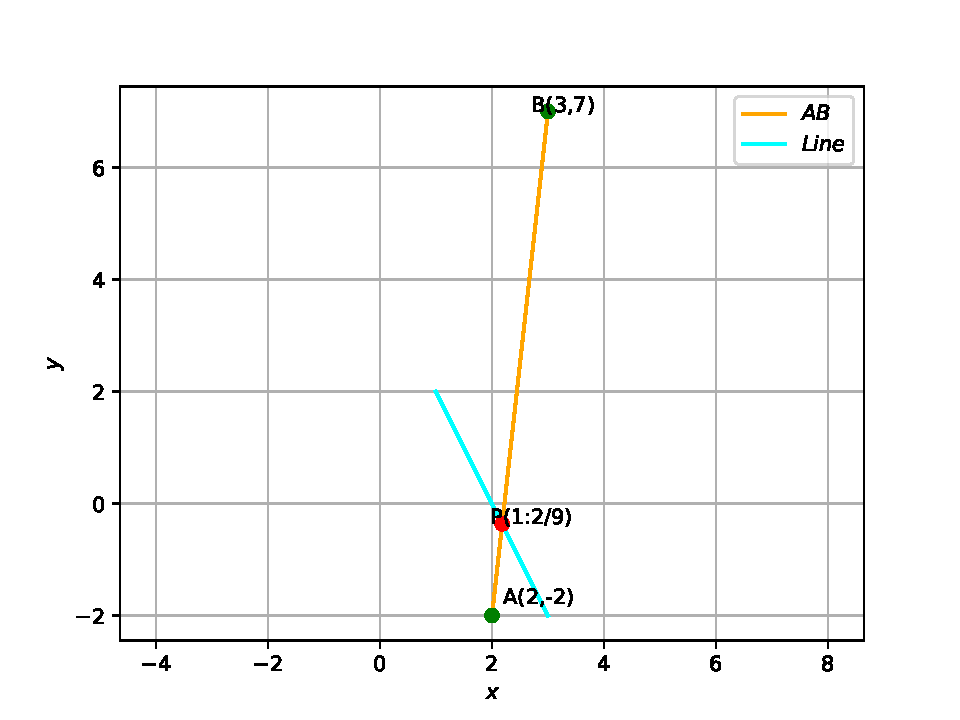
\includegraphics[width=\columnwidth]{chapters/10/7/4/1/figs/vec.pdf}
\caption{}
\label{fig:chapters/10/7/4/1vec}
\end{figure}


\item Let $\vec{A}(4, 2), \vec{B}(6, 5)$  and $ \vec{C}(1, 4)$ be the vertices of $\triangle ABC$.
\begin{enumerate}
\item The median from $\vec{A}$ meets $BC$ at $\vec{D}$. Find the coordinates of the point $\vec{D}$.
\item Find the coordinates of the point $\vec{P}$ on $AD$ such that $AP : PD = 2 : 1$.
\item Find the coordinates of points $\vec{Q}$ and $\vec{R}$ on medians $BE$ and $CF$ respectively such that $BQ : QE = 2 : 1$  and  $CR : RF = 2 : 1$.
\item What do you observe?
\item If $\vec{A}, \vec{B}$ and $\vec{C}$  are the vertices of $\triangle ABC$, find the coordinates of the centroid of the triangle.
\end{enumerate}
\solution
	\iffalse
\documentclass[12pt]{article}
\usepackage{graphicx}
\usepackage[none]{hyphenat}
\usepackage{graphicx}
\usepackage{listings}
\usepackage[english]{babel}
\usepackage{graphicx}
\usepackage{caption} 
\usepackage{booktabs}
\usepackage{array}
\usepackage{amssymb} % for \because
\usepackage{amsmath}   % for having text in math mode
\usepackage{extarrows} % for Row operations arrows
\usepackage{listings}
\usepackage[utf8]{inputenc}
\lstset{
  frame=single,
  breaklines=true
}
\usepackage{hyperref}
  
%Following 2 lines were added to remove the blank page at the beginning
\usepackage{atbegshi}% http://ctan.org/pkg/atbegshi
\AtBeginDocument{\AtBeginShipoutNext{\AtBeginShipoutDiscard}}


%New macro definitions
\newcommand{\mydet}[1]{\ensuremath{\begin{vmatrix}#1\end{vmatrix}}}
\providecommand{\brak}[1]{\ensuremath{\left(#1\right)}}
\newcommand{\solution}{\noindent \textbf{Solution: }}
\newcommand{\myvec}[1]{\ensuremath{\begin{pmatrix}#1\end{pmatrix}}}
\providecommand{\norm}[1]{\left\lVert#1\right\rVert}
\providecommand{\abs}[1]{\left\vert#1\right\vert}
\let\vec\mathbf

\begin{document}

\begin{center}
\title{\textbf{VECTORS}}
\date{\vspace{-5ex}} %Not to print date automatically
\maketitle
\end{center}

\section{10$^{th}$ Maths - EXERCISE-7.4}

Let A(4, 2), B(6, 5) and C(1, 4) be the vertices of $\triangle ABC$
\begin{enumerate}
\item The median from A meets BC at D. Find the coordinates of the point D.
\item Find the coordinates of the point P on AD such that $AP : PD = 2 : 1$
\item Find the coordinates of points Q and R on medians BE and CF respectively such
that $BQ : QE = 2 : 1 \text{and} CR : RF = 2 : 1.$
\item What do yo observe?
\item If $A(x_1, y_1), B(x_2, y_2) \text{and} C(x_3, y_3)$ are the vertices of $\triangle ABC$, find the coordinates of the centroid of the triangle.
\end{enumerate}

Given points are
\begin{align}
\vec{A}=\myvec{4\\ 2} ,
\vec{B}=\myvec{6\\ 5} ,
\vec{C}=\myvec{1\\ 4}
\end{align}
\fi

\begin{enumerate}
\item 
\begin{align}
\vec{D}&=\frac{\vec{B}+\vec{C}}{2}\\
&=\myvec{\frac{7}{2}\\[2pt] \frac{9}{2}}\\
\vec{E}&=\frac{\vec{A}+\vec{C}}{2}\\
&=\myvec{\frac{5}{2}\\ 3}\\
\vec{F}&=\frac{\vec{A}+\vec{B}}{2}\\
&=\myvec{5\\ \frac{7}{2}}
\end{align}

\item 
	For
$n=2$,
\begin{align}
\vec{P}&=\frac{1}{1+n}\brak{\myvec{\vec{A}+n\vec{D}}}\\
&=\frac{1}{3}\myvec{11\\11}
\end{align}

\item 
\begin{align}
\vec{Q}&=\frac{1}{1+n}\brak{\myvec{\vec{B}+n\vec{E}}}\\
&=\frac{1}{3}\myvec{11\\11}\\
\vec{R}&=\frac{1}{1+n}\brak{\myvec{\vec{C}+n\vec{F}}}\\
&=\frac{1}{3}\myvec{11\\11}\\
\end{align}

\item 
 $\vec{P},\vec{Q},\vec{R}$ are the same point.
   
\item 
\begin{align}
\vec{G}&=\frac{\vec{D}+\vec{E}+\vec{F}}{3}\\
&=\frac{1}{3}\myvec{11\\11}\\
\end{align} 
\end{enumerate}
See Fig.  
  \ref{fig:chapters/10/7/4/7/Figure}.
\begin{figure}[h!]
\centering
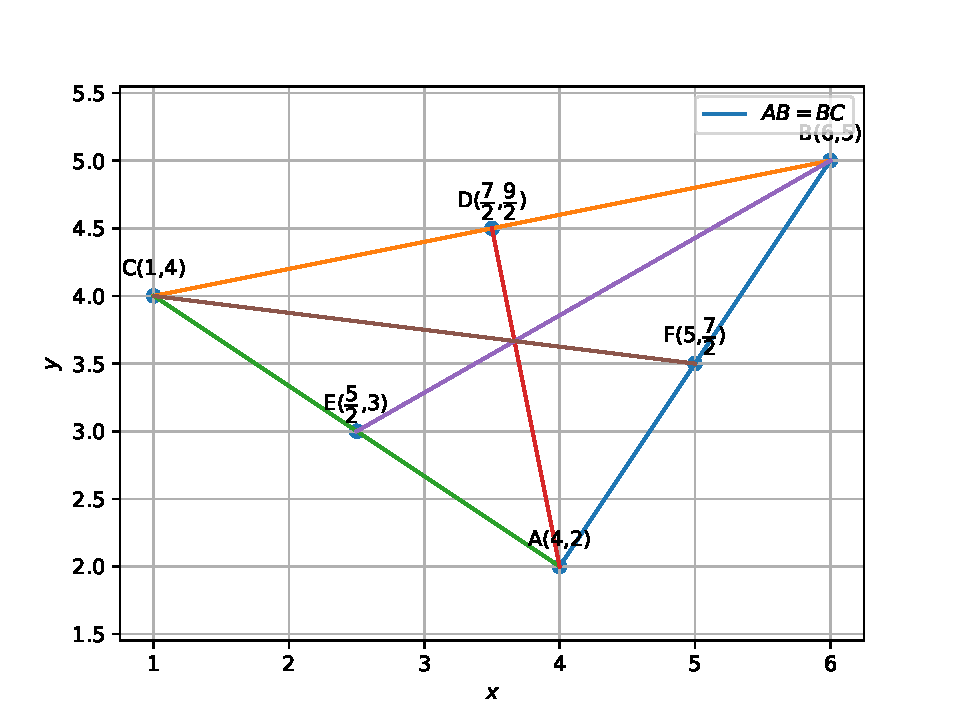
\includegraphics[width=\columnwidth]{chapters/10/7/4/7/figs/dj.pdf}
\caption{}
  \label{fig:chapters/10/7/4/7/Figure}
\end{figure}

\item Find the position vector of a point R which divides the line joining two points $P$ and $Q$ whose position vectors are $(2\vec{a}+\vec{b})$ and $(\vec{a}-3\vec{b})$
externally in the ratio 1 : 2. Also, show that $P$ is the mid point of the line segment $RQ$.\\
	\solution
		\iffalse
\documentclass[10pt]{article}
\usepackage{graphicx}
\usepackage[none]{hyphenat}
\usepackage{graphicx}
\usepackage{listings}
\usepackage[english]{babel}
\usepackage{siunitx}
\usepackage{graphicx}
\usepackage{caption} 
\usepackage{booktabs}
\usepackage{array}
\usepackage{amssymb} % for \because
\usepackage{amsmath}   % for having text in math mode
\usepackage{extarrows} % for Row operations arrows
\usepackage{listings}
\usepackage[utf8]{inputenc}
\lstset{
  frame=single,
  breaklines=true
}
\usepackage{hyperref}
  
%Following 2 lines were added to remove the blank page at the beginning
\usepackage{atbegshi}% http://ctan.org/pkg/atbegshi
\AtBeginDocument{\AtBeginShipoutNext{\AtBeginShipoutDiscard}}


%New macro definitions
\newcommand{\mydet}[1]{\ensuremath{\begin{vmatrix}#1\end{vmatrix}}}
\providecommand{\brak}[1]{\ensuremath{\left(#1\right)}}
\newcommand{\solution}{\noindent \textbf{Solution: }}
\newcommand{\myvec}[1]{\ensuremath{\begin{pmatrix}#1\end{pmatrix}}}
\providecommand{\norm}[1]{\left\lVert#1\right\rVert}
\providecommand{\abs}[1]{\left\vert#1\right\vert}
\let\vec\mathbf{}
\begin{document}

\begin{center}
\title{\textbf{VECTORS}}
\date{\vspace{-5ex}} %Not to print date automatically
\maketitle
\end{center}

\section*{12$^{th}$ Maths - EXERCISE-10.5}

Find the position vector of a point R which divides the line joining two points  P and Q whose position vectors are P = $\myvec{2\\ 1 \\}$ and Q = $\myvec{ 1\\-3\\ }$  externally in the ratio 1:2.Also show that P is the midpoint of the linesegment RQ.

\solution

\begin{align}
\vec{P} = \myvec{ 2\\1\\} 
 \label{eq1} \\
 \vec{Q} = \myvec{ 1\\-3\\}
\end{align}
\fi
When $\vec{R}$ divides line segment joining $\vec{P}$ and $\vec{Q}$ externally,
\begin{align}
\vec{R} &= \frac{\vec{Q} -2\vec{P}}{-1} 
= \myvec{3\\5}
\end{align}
Also,
\begin{align}
\frac{ (\vec{R} + \vec{Q})}{2}
=\myvec{2\\1} =\vec{P}
\end{align}
See Fig. 
\ref{fig:chapters/12/10/5/9/Figure1}.
\begin{figure}[!h]
	\begin{center}
		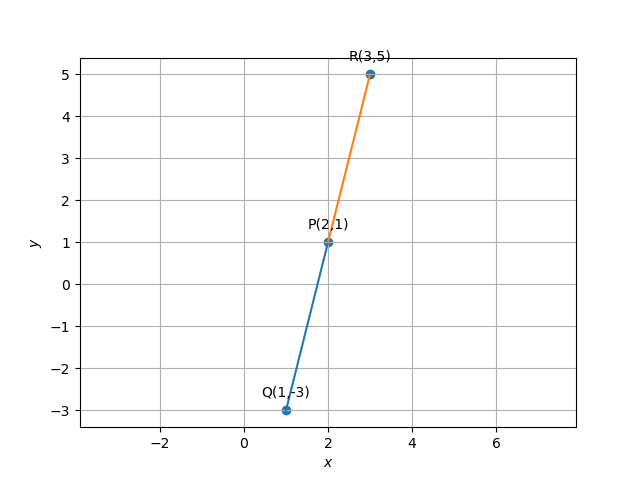
\includegraphics[width=\columnwidth]{chapters/12/10/5/9/figs/line.png}
	\end{center}
\caption{}
\label{fig:chapters/12/10/5/9/Figure1}
\end{figure}

\item The point which divides the line segment joining the points $\vec{P} (7, –6) $  and  $\vec{Q}(3, 4)$ in the 
ratio 1 : 2 internally lies in the
\begin{enumerate}
\item I quadrant
\item  II quadrant
\item  III quadrant
\item  IV quadrant
\end{enumerate}
\item If the point $\vec{P} (2, 1)$ lies on the line segment joining points $\vec{A} (4, 2)$  and $ \vec{B} (8, 4)$,
then
\begin{enumerate}
	\item $AP =\frac{1}{3}{AB}$ 
\item ${AP}={PE}$
\item ${PB}=\frac{1}{3}{AB}$
\item${AP}=\frac{1}{2}{AB}$
 \end{enumerate}
\item A line intersects the y-axis and x-axis at the points $\vec{P}$  and $\vec{Q}$, respectiveiy. lf $(2,5)$ is the mid-point of $\vec{PQ}$, then the coordinates of $\vec{P}$ and $ \vec{Q}$ are, respectively
\begin{enumerate}
	\item$(0,-5)$ and $(2,0)$
	\item$(0,-10)$ and $(-4,0)$
	\item$(0,4)$ and  $(-10,0)$
	\item$(0,-10)$ and $(4,0)$
\end{enumerate}
\item Point $\vec{P}(5,-3)$ is one of the two points of trisection of line segment joining the points $\vec{A}(7,-2)\text{ and }\vec{B}(1,-5)$
\item Points $\vec{A}(-6,10),\vec{B}(-4,6) \text{ and } \vec{C}(3,-8)$ are collinear such that $\vec{A}\vec{B}=  \frac{2}{9}\vec{A}\vec{C}$
\item In what ratio does the $x$-axis divide the line segment joining the points $(-4,-6)\text{ and }(-1,7)$? Find the coordinates of the point of division.
\item Find the ratio in which the point $\vec{P}\brak{\frac{3}{4},\frac{5}{12}}$ divides the line segment joining the points $\vec{A}\brak{\frac{1}{2},\frac{3}{2}}\text{ and } \vec{B}(2,-5)$.
\item If $\vec{P}(9a-2,-b)$ divides line segment joining $\vec{A}(3a+1,-3)\text{ and }\vec{B}(8a,5)$ in the ratio 3:1, find the values of $a$ and $b$.
\item The line segment joining the points $\vec{A}(3,2)\text{ and }\vec{B}(5,1)$ is divided at the point $\vec{P}$ in the ratio 1:2 which lies on $3x-18y+k=0$. Find the value of $k$.  
\item Find the coordinates of the point $\vec{R}$ on the line segment joining the points $\vec{P}(-1,3)\text{ and }\vec{Q}(2,5)$ such that $PR=\frac{3}{5}PQ$.
\item Find the ratio in which the line $2x+3y-5=0$ divides the line segment joining the points $(8,-9)$ and $(2,1)$. Also find the coordinates of the point of division.
\item If $\vec{a}$ and $\vec{b}$ are the postion vectors of $A$ and $B$, respectively, find the position vector of a point $C$ in $BA$ produced such that $BC=1.5BA$.
\item The position vector of the point which divides the join of points 2$\vec{a}$-3$\vec{b}$ $\text{and}$ $\vec{a}+\vec{b}$ in the ratio 3:1 is
	\begin{enumerate}
\item $\frac{3\vec{a}-2\vec{b}}{2}$
\item $\frac{7\vec{a}-8\vec{b}}{4}$
\item $\frac{\vec{3a}}{4}$
\item $\frac{\vec{5a}}{4}$
\end{enumerate}
\item Find the ratio in which the line segment joining $A(1,-5) \text{ and } B(-4,5)$ $\text{is divided by the x-axis}$. Also find the coordinates of the point of division.
\item Find the position vector of a point $\vec{R}$ which divides the line joining two points $\vec{P}$ and $\vec{Q}$ whose position vectors are $2\vec{a}+\vec{b}$ and $\vec{a}-3\vec{b}$ externally in the ratio $1:2$.
\end{enumerate}

